
\documentclass[a4paper,USenglish]{oasics-v2016}

\usepackage{microtype}
\bibliographystyle{plainurl}

\usepackage[utf8]{inputenc}
\usepackage{amsmath,amssymb}
\usepackage{url}
\usepackage{wrapfig}
\usepackage{listings}
\usepackage{xcolor}
\usepackage{graphicx}

\frenchspacing
\renewcommand{\topfraction}{1}
\renewcommand{\bottomfraction}{1}

\lstset{xleftmargin=2\parindent,aboveskip=\smallskipamount,belowskip=\smallskipamount,captionpos=b}
\lstset{numbers=left,numberblanklines=false,basicstyle=\ttfamily\small}
\lstset{keywords=[1]{m,n},keywordstyle=[1]\usefont{OT1}{cmtt}{m}{n}}

\lstdefinelanguage{clingo}{
  keywordstyle=[1]\usefont{OT1}{cmtt}{m}{n},%
  keywordstyle=[2]\textbf,%
  keywordstyle=[3]\usefont{OT1}{cmtt}{m}{n},%
  alsoletter={\#,\&},%
  keywords=[1]{not,from,import,def,if,else,return,while,break,and,or,for,in,del,and,class},%
  keywords=[2]{\#const,\#show,\#minimize,\#base,\#theory,\#count,\#external,\#program,\#script,\#end,\#heuristic,\#edge,\#project,\#show},%
  keywords=[3]{&,&dom,&sum,&diff,&show},%
  morecomment=[l]{\#\ },%
  morecomment=[l]{\%\ },%
  commentstyle={\color{darkgray}}%
}

\newcommand{\naf}[1]{\ensuremath{{\sim}{#1}}}
\newcommand{\poslits}[1]{\ensuremath{#1^+}}
\newcommand{\neglits}[1]{\ensuremath{#1^-}}
\newcommand{\body}[1]{\ensuremath{B(#1)}} 
\newcommand{\pbody}[1]{\poslits{\body{#1}}} 
\newcommand{\nbody}[1]{\neglits{\body{#1}}} 
\newcommand{\head}[1]{\ensuremath{h(#1)}} 

\newcommand{\Tsign}{\ensuremath{\mathbf{T}}}
\newcommand{\Fsign}{\ensuremath{\mathbf{F}}}
\newcommand{\Tlit}[1]{\ensuremath{\Tsign #1}}
\newcommand{\Flit}[1]{\ensuremath{\Fsign #1}}
\newcommand{\Ass}{\ensuremath{\mathbf{A}}}
\newcommand{\DL}{\ensuremath{\mathit{DL}}}

\newcommand{\code}[1]{{\ttfamily #1}}
\newcommand{\codeClass}[2]{\code{#2}}

\newcommand{\sysfont}{\textit}
\newcommand{\acthex}{\sysfont{acthex}}
\newcommand{\asparagus}{\sysfont{asparagus}}
\newcommand{\aspic}{\sysfont{aspic}}
\newcommand{\aspmt}{\sysfont{aspmt}}
\newcommand{\asprin}{\sysfont{asprin}}
\newcommand{\assat}{\sysfont{assat}}
\newcommand{\berkmin}{\sysfont{berkmin}}
\newcommand{\claspD}{\sysfont{claspD}}
\newcommand{\claspar}{\sysfont{claspar}}
\newcommand{\claspfolio}{\sysfont{claspfolio}}
\newcommand{\clasp}{\sysfont{clasp}}
\newcommand{\clingcon}{\sysfont{clingcon}}
\newcommand{\clingo}{\sysfont{clingo}}
\newcommand{\cmodels}{\sysfont{cmodels}}
\newcommand{\coala}{\sysfont{coala}}
\newcommand{\dingo}{\sysfont{dingo}}
\newcommand{\dflat}{\sysfont{dflat}}
\newcommand{\dlvhex}{\sysfont{dlvhex}}
\newcommand{\dlv}{\sysfont{dlv}}
\newcommand{\ezcsp}{\sysfont{ezcsp}}
\newcommand{\ftolp}{\sysfont{f2lp}}
\newcommand{\gecode}{\sysfont{gecode}}
\newcommand{\gidl}{\sysfont{gidl}\xspace}
\newcommand{\gnt}{\sysfont{gnt}}
\newcommand{\gringo}{\sysfont{gringo}}
\newcommand{\iclingo}{\sysfont{iclingo}}
\newcommand{\idp}{\sysfont{idp}}
\newcommand{\inca}{\sysfont{inca}}
\newcommand{\jdlv}{\sysfont{jdlv}}
\newcommand{\lparse}{\sysfont{lparse}}
\newcommand{\lptodiff}{\sysfont{lp2diff}}
\newcommand{\lptosat}{\sysfont{lp2sat}}
\newcommand{\lctocasp}{\sysfont{lc2casp}}
\newcommand{\mchaff}{\sysfont{mchaff}}
\newcommand{\metasp}{\sysfont{metasp}}
\newcommand{\mingo}{\sysfont{mingo}}
\newcommand{\minisat}{\sysfont{minisat}}
\newcommand{\nomorepp}{\sysfont{nomore++}}
\newcommand{\oclingo}{\sysfont{oclingo}}
\newcommand{\piclasp}{\sysfont{piclasp}}
\newcommand{\picosat}{\sysfont{picosat}}
\newcommand{\plasp}{\sysfont{plasp}}
\newcommand{\quontroller}{\sysfont{quontroller}}
\newcommand{\rosoclingo}{\sysfont{rosoclingo}}
\newcommand{\sag}{\sysfont{sag}}
\newcommand{\satz}{\sysfont{satz}}
\newcommand{\siege}{\sysfont{siege}}
\newcommand{\smodelscc}{\sysfont{smodels$_{\!cc}$}}
\newcommand{\smodelsr}{\sysfont{smodels}$_r$}
\newcommand{\smodels}{\sysfont{smodels}}
\newcommand{\unclasp}{\sysfont{unclasp}}
\newcommand{\wasp}{\sysfont{wasp}}
\newcommand{\zchaff}{\sysfont{zchaff}}
\newcommand{\zzz}{\sysfont{z3}}

\newcommand{\aspif}{\sysfont{aspif}}

\newcommand{\python}{Python}
\newcommand{\lua}{Lua}
\newcommand{\cpp}{C++}
\newcommand{\C}{C}
\newcommand{\java}{Java}
\newcommand{\haskell}{Haskell}

\newcommand{\neghspace}{\!\!\!\!\!}

\title{Theory Solving Made Easy with \textit{Clingo}~5\footnote{This work was partially supported by DFG-SCHA-550/9}}
\titlerunning{Theory Solving Made Easy with \textit{Clingo}~5}

\author[1]{Martin~Gebser}
\author[1]{Roland~Kaminski}
\author[1]{Benjamin~Kaufmann}
\author[1]{Max~Ostrowski}
\author[1,2]{Torsten~Schaub}
\author[1]{Philipp~Wanko}

\affil[1]{University of Potsdam, Germany}
\affil[2]{INRIA Rennes, France}

\authorrunning{M. Gebser, R. Kaminski, B. Kaufmann, M. Ostrowski, T. Schaub, and P. Wanko}

\Copyright{M. Gebser, R. Kaminski, B. Kaufmann, M. Ostrowski, T. Schaub, and P. Wanko}

\subjclass{D.1.6 Logic Programming}
\keywords{Answer Set Programming, Theory Language, Theory Propagation}

\pdfinfo{
/Title (Theory Solving Made Easy with Clingo 5)
/Author (Martin~Gebser, Roland~Kaminski, Benjamin~Kaufmann, Max~Ostrowski, Torsten~Schaub, Philipp~Wanko) }

\EventEditors{Manuel Carro, Andy King, Marina De Vos, and Neda Saeedloei}
\EventNoEds{4}
\EventLongTitle{Technical Communications of the 32nd Int'l Conference on Logic
      Programming (ICLP 2016)}
\EventShortTitle{ICLP 2016 TCs}
\EventAcronym{ICLP}
\EventYear{2016}
\EventDate{October 16--21, 2016}
\EventLocation{New York City, USA}
\EventLogo{}
\SeriesVolume{52}
\ArticleNo{NNN}

\begin{document}

\maketitle

\begin{abstract}
Answer Set Programming (ASP) is a model, ground, and solve paradigm.
The integration of application- or theory-specific reasoning into ASP systems thus impacts on many if not all elements of its workflow,
viz.\
input language,
grounding,
intermediate language,
solving, and
output format.
%
We address this challenge with the fifth generation of the ASP system \clingo\ and its grounding and solving components
by equipping them with well-defined generic interfaces facilitating the manifold integration efforts.
%
On the grounder's side, we introduce a generic way of specifying language extensions and 
propose an intermediate format accommodating their ground representation.
At the solver end, this is accompanied by high-level interfaces 
easing the integration of theory propagators dealing with these extensions.
\end{abstract}


\section{Introduction}\label{sec:introduction}

The \clingo\ system, along with its grounding and solving components \gringo\ and \clasp, %
is  nowadays among the most widely used tools for Answer Set Programming (ASP; \cite{lifschitz08b}).
This does not only apply to end-users, but more and more to system developers who build upon \clingo's
infrastructure for developing their own systems.
Among them, we find (alphabetically)
\clasp\emph{-nk}~\cite{eiererfi13a},
\clingcon~\cite{ostsch12a},
\dflat~\cite{abblchduhewo14a},
\dingo~\cite{jalini11a},
\dlvhex~\cite{eifikrre12a},
\inca~\cite{drewal12a}, and
\mingo~\cite{lijani12a}.
None of these systems can use \clingo\ or its components without workarounds or even involved modifications to realize the desired functionality.
%
Moreover, since ASP is a model, ground, and solve paradigm, such modifications are rarely limited to a single component
but often spread throughout the whole workflow.
This begins with the addition of new language constructs to the input language,
requiring in turn amendments to the grounder as well as
syntactic means for passing the ground constructs to a downstream system.
In case they are to be dealt with by an ASP solver,
it must be enabled to treat the specific input and incorporate corresponding solving capacities.
%
Finally,
each such extension is application-specific and requires different means at all ends.

We address this challenge with the new \clingo\ series~5 and its components.
%
This is accomplished by introducing generic interfaces that allow for accommodating extensions to ASP at the salient stages of its workflow.
%
To begin with,
we extend \clingo's grounder component \gringo\ with means for specifying simple theory grammars in which new theories can be represented.
As theories are expressed using constructs close to ASP's basic modeling language,
the existing grounding machinery takes care of instantiating them.
%
This also involves a new intermediate ASP format that allows for passing the enriched information from grounders to solvers in a transparent way.
(Since this format is mainly for settings with stand-alone grounders and solvers,
 and thus outside the scope of \clingo,
 we delegate details to~\cite{gekakaosscwa16b}.) %
%
For a complement,
\clingo~5 provides several interfaces for reasoning with theory expressions.
%
On the one hand,
the existing \lua\ and \python\ APIs are extended by high-level interfaces for
augmenting propagation in \clasp\ with so-called \emph{theory propagators}.
Several such propagators can be registered with \clingo,
each implementing an interface of four basic methods.
Our design is driven by the objective to provide means for rapid prototyping of dedicated reasoning procedures while enabling effective implementations.
To this end,
the interface supports, for instance, stateful theory propagators as well as multi-threading in the underlying solver.
%
On the other hand,
the functionality of the aforementioned extended APIs is now also offered via a \C\ interface.
This is motivated by the wide availability of foreign function interfaces for \C, which enable the import of \clingo\ %
in %
programming languages like \java\ or \haskell.
A first application of this is the integration of \clingo~5 into SWI-Prolog.\footnote{\url{https://github.com/JanWielemaker/clingo}}

\section{Input Language}\label{sec:language}

This section introduces the novel features of \clingo~5's input language.
All of them are situated in the underlying grounder \gringo~5 and can thus
also be used independently of \clingo.
%
We start with a detailed description of \gringo~5's generic means for defining theories
and afterwards summarize further %
new features.

Our generic approach to theory specification rests upon two languages:
the one defining theory languages and the theory language itself.
Both borrow elements from the underlying ASP language,
foremost an aggregate-like syntax for formulating variable length expressions.
To illustrate this, consider Listing~\ref{prg:diff},
where a logic program is extended by constructs for handling difference and linear constraints.
While the former are binary constraints of the form $x_1-x_2\leq k$, %
the latter have a variable size and are of form
\(
a_1x_1+\dots+a_nx_n\circ k
\),
where $x_i$ are integer variables, $a_i$ and $k$ are integers, and $\circ\in\{\leq,\geq,<,>,=\}$
for $1\leq i\leq n$.%
\footnote{For simplicity, we consider normalized difference constraints rather than general ones of form $x_1-x_2\circ k$.}
Note that solving difference constraints is polynomial, while solving linear equations (over integers) is NP-hard.
The theory language for expressing both types of constraints is defined in Lines~\ref{prg:diff:begin-theory}--\ref{prg:diff:end-theory} and preceded by the directive \lstinline{#theory}.
The elements of the resulting theory language are preceded by \lstinline{&} and used as regular atoms in the logic program in Lines~\ref{prg:diff:begin-program}--\ref{prg:diff:end-program}.
%
\lstinputlisting[language=clingo,morekeywords={n,m},float=t,escapeinside={\%(}{\%)},basicstyle=\ttfamily\small,label=prg:diff,caption=Logic program enhanced with difference and linear constraints (\texttt{diff.lp})]{code/diff.lp}


To be more precise,
a \emph{theory definition} has the form
\begin{lstlisting}[numbers=none,mathescape=t]
#theory $T$ {$D_1$;$\dots$;$D_n$}.
\end{lstlisting}
where $T$ is the theory name and each $D_i$ is a definition for a theory term or a theory atom for $1\leq i\leq n$.
The language induced by a theory definition is the set of all theory atoms constructible from its theory atom definitions.

A \emph{theory atom definition} has form
\begin{lstlisting}[numbers=none,mathescape=t]
&$p$/$k$ : $t$,$o$ $\quad\textrm{ or }\quad$ &$p$/$k$ : $t$,{$\diamond_1$,$\dots$,$\diamond_m$},$t'$,$o$
\end{lstlisting}
where $p$ is a predicate name and $k$ its arity,
$t,t'$ are names of theory term definitions,
each $\diamond_i$ is a theory operator for $m\geq 1$,
and
\(
o\in\{\mathtt{head},\mathtt{body},\mathtt{any}, \mathtt{directive}\}
\)
determines where theory atoms may occur in a rule.
%
Examples of theory atom definitions are given in Lines~\ref{lst:ex1-begin-def-atom}--\ref{lst:ex1-end-def-atom} of Listing~\ref{prg:diff}.
%
The language of a theory atom definition as above contains all \emph{theory atoms} of form
\begin{lstlisting}[numbers=none,mathescape=t]
&$a$ {${C}_1$:${L}_1$;$\dots$;${C}_n$:${L}_n$}$\quad\textrm{ or }\quad$ &$a$ {${C}_1$:${L}_1$;$\dots$;${C}_n$:${L}_n$} $\diamond$ $c$
\end{lstlisting}
where $a$ is an atom over predicate $p$ of arity $k$,
each ${C}_i$ is a tuple of theory terms in the language for~$t$,
$c$ is a theory term in the language for~$t'$,
$\diamond$ is a theory operator among $\{ \diamond_1, \dots, \diamond_m \}$,
and each ${L}_i$ is a regular condition (i.e., a tuple of regular literals)
for $1\leq i\leq n$.
%
Whether the last part `${}\diamond c$' is included depends on the form of a theory atom definition.
%
Five occurrences of theory atoms can be found in Lines~\ref{prg:diff:begin-use-theory}--\ref{prg:diff:end-use-theory} of Listing~\ref{prg:diff}.

A \emph{theory term definition} has form
\begin{lstlisting}[numbers=none,mathescape=t]
$t$ {$D_1$;$\dots$;$D_n$}
\end{lstlisting}
where $t$ is a name for the defined terms and each $D_i$ is a theory operator definition 
for $1\leq i\leq n$.
A respective definition specifies the language of all theory terms
that can be constructed via %
its operators. %
%
Examples of theory term definitions are given in Lines~\ref{prg:diff:begin-def-term}--\ref{prg:diff:end-def-term} of Listing~\ref{prg:diff}.
%
Each resulting \emph{theory term} is one of the following:
\par\medskip\noindent
\begin{minipage}{0.5\linewidth}
  \begin{itemize}
  \item a constant term: \ $c$
  \item a variable term: \ $v$
  \item a binary theory term: \  $t_1 \diamond t_2$
  \item a unary theory term: \  ${}\diamond t_1$
  \end{itemize}
\end{minipage}
\begin{minipage}{0.5\linewidth}
\begin{itemize}
  \item a function theory term: \  $f(t_1,\dots,t_k)$
  \item a tuple theory term: \  $(t_1,\dots,t_l,)$
  \item a set theory term: \  $\{t_1,\dots,t_l\}$
  \item a list theory term: \  $[t_1,\dots,t_l]$
\end{itemize}
\end{minipage}
\par\medskip\noindent
where each $t_i$ is a theory term,
$\diamond$ is a theory operator defined by some $D_i$,
$c$ and $f$ are symbolic constants,
$v$ is a first-order variable,
$k\geq 1$, and
$l\geq 0$.
(The trailing comma in tuple theory terms is optional if $l \neq 1$.)
%
Parentheses can be used to specify operator precedence.

A \emph{theory operator definition} has form
\begin{lstlisting}[numbers=none,mathescape=t]
$\diamond$ : $p$,unary $\quad\textrm{ or }\quad$ $\diamond$ : $p$,binary,$a$
\end{lstlisting}
where $\diamond$ is a unary or binary theory operator with precedence $p\geq 0$
(determining implicit parentheses). %
Binary theory operators are additionally characterized by an associativity
$a\in\{\text{\lstinline{right}},\linebreak[1]\text{\lstinline{left}}\}$.
%
As an example,
consider Line~\ref{prg:diff:op-mul} of Listing~\ref{prg:diff},
where the \lstinline{binary} operator~\lstinline{*} is defined with precedence~\lstinline{1} and \lstinline{left} associativity.
%
In total, Lines~\ref{prg:diff:begin-def-term}--\ref{prg:diff:end-def-term} of Listing~\ref{prg:diff}
include nine theory operator definitions.
%
Particular \emph{theory operators} can be assembled (written consecutively without spaces) from the symbols
`\lstinline{!}',
`\lstinline{<}',
`\lstinline{=}',
`\lstinline{>}',
`\lstinline{+}',
`\lstinline{-}',
`\lstinline{*}',
`\lstinline{/}',
`\lstinline{\}',
`\lstinline{?}',
`\lstinline{&}',
%
`\lstinline{|}',
`\lstinline{.}',
`\lstinline{:}',
`\lstinline{;}',
`\lstinline{~}', and
`\lstinline{^}'.
%
For instance,
in Line~\ref{prg:diff:op-dot} of Listing~\ref{prg:diff}, the operator `\lstinline{..}' is defined as the concatenation of two periods.
%
%
The tokens
`\lstinline{.}',
`\lstinline{:}',
`\lstinline{;}', and
`\lstinline{:-}'
must be combined with other symbols
due to their dedicated usage.
Instead, one may write
`\lstinline{..}',
`\lstinline{::}',
`\lstinline{;;}',
`\lstinline{::-}',
etc.

While theory terms are formed similar to regular ones,
theory atoms rely upon an aggregate-like construction for forming variable-length theory expressions.
In this way, standard grounding techniques can be used for gathering theory terms.
(However, the actual atom within a theory atom comprises regular terms only.)
%
The treatment of theory terms still %
differs from their regular counterparts
%
in that the grounder skips simplifications like, e.g., arithmetic evaluation.
%
This can be nicely seen on the different results in Listing~\ref{prg:grd:diff} of grounding terms formed with
the regular and theory-specific variants of operator `\lstinline{..}'.
Observe that
the     fact \lstinline{task(1..n)} in Line~\ref{prg:diff:rule-task} of Listing~\ref{prg:diff} results in \lstinline{n} ground     facts,
viz.\ \lstinline{task(1)} and \lstinline{task(2)} because of \lstinline{n=2}.
Unlike this, the theory expression \lstinline{1..m} stays structurally intact and is only transformed into \lstinline{1..1000} in view of \lstinline{m=1000}.
That is, the grounder does not evaluate the theory term \lstinline{1..1000} and
leaves its interpretation to a downstream theory solver.
%
\lstinputlisting[language=clingo,float=t,basicstyle=\ttfamily\small,label=prg:grd:diff,caption={Human-readable result of grounding Listing~\ref{prg:diff} via `\texttt{gringo --text diff.lp}'}]{code/diff.grd}
%
%
A similar situation is encountered when comparing the treatment of the regular term `\lstinline{200*T}' in Line~\ref{prg:diff:rule-duration} of Listing~\ref{prg:diff} to the
theory term `\lstinline{end(T)-start(T)}' in Line~\ref{prg:diff:rule-diff}.
While each instance of `\lstinline{200*T}' is evaluated during grounding,
instances of the theory term  are left in Line~6 of Listing~\ref{prg:grd:diff}.
In fact, if `\lstinline{200*T}' had been a theory term as well,
it would have resulted in the unevaluated instances  `\lstinline{200*1}' and `\lstinline{200*2}'. %


The remainder of this section is dedicated to other language extensions of \gringo~5 aiming
at a disentanglement of the various uses of \lstinline{#show} directives
(and their induced symbol table).
Such directives were beforehand used for
controlling the output of stable models,
delineating the scope of reasoning modes (e.g., intersection, union, projection, etc.),
and for
passing special-purpose information to downstream systems.
For instance,
theory and heuristic information was passed to \clasp\ via dedicated predicates like \lstinline{_edge} and \lstinline{_heuristic}.
This entanglement brought about several shortcomings.
%
In fact, passing information via a symbol table did not only scramble the output, but also provoked overhead in grounding and filtering ``artificial'' symbolic information.

Now, in \gringo~5, the sole purpose of \lstinline{#show} is to furnish an output directive.
There are three different kinds of such statements:
%
\begin{lstlisting}[numbers=none,mathescape=t]
#show.     #show $p$/$n$.      #show $t$ : $l_1$,$\dots$,$l_n$.
\end{lstlisting}
%
The first form hides all atoms, and the second all except those over predicates~$p/n$ indicated by \lstinline{#show} statements.
The third form does not hide any atoms and can be used to output arbitrary terms~$t$,
whenever the literals $l_1,\dots,l_n$ in the condition after~`\lstinline{:}' hold.
This is particularly useful in meta-programming,
e.g., `\lstinline{#show A : holds(A).}' can be used to map back reified atoms.

Atoms used in reasoning modes are indicated by \lstinline{#project} directives, having two forms:
%
\begin{lstlisting}[numbers=none,mathescape=t]
#project $p$/$n$.     #project $a$ : $l_1$,$\dots$,$l_n$.
\end{lstlisting}
%
Here, $p$ is a predicate name with arity $n$, $a$ is an atom, and $l_1,\dots,l_n$ are %
literals.
While the first form declares all atoms over predicate~$p/n$ as %
subject to projection,
the second includes instances of~$a$
obtained via grounding, as detailed in \cite{gekakasc14b} for
\lstinline{#external} directives.

The last two new directives of interest abolish the need for %
the special-purpose predicates \lstinline{_edge} and \lstinline{_heuristic},
previously used in conjunction with the ASP solver \clasp:
\begin{lstlisting}[numbers=none,mathescape=t]
#edge ($u$,$v$) : $l_1$,$\dots$,$l_n$.
#heuristic $a$ : $l_1$,$\dots$,$l_n$. [$k$@$p$,$m$]
\end{lstlisting}
As above, $a$ is an atom, and $l_1,\dots,l_n$ are literals.
Moreover,
$u,v,k,p,m$ are terms, %
where 
`\lstinline[mathescape=t]{($u$,$v$)}' stands for an
edge from $u$ to $v$ in an acyclicity extension \cite{bogejakasc15a}.
Integer values for $k$ and $p$ along with
\lstinline{init}, \lstinline{factor}, \lstinline{level}, \lstinline{sign}, \lstinline{true}, or \lstinline{false} for~$m$
determine a heuristic modifier \cite{gekaotroscwa13a}.
Finally, note that
zero is taken as default priority when
the optional `\lstinline[mathescape=t]{@$p$}' part 
in `\lstinline[mathescape=t]{[$k$@$p$,$m$]}',
resembling the syntax of ranks for weak constraints \cite{aspcore2},
is omitted.

\section{Logical Characterization}
\label{sec:foundations}

The semantics of logic programs modulo theories rests upon
ground programs~$P$ over two disjoint alphabets, $\mathcal{A}$ and $\mathcal{T}$,
consisting of regular and \emph{theory atoms}. %
Accordingly, $P$ is a set of rules~$r$ of the form
$h \leftarrow a_1,\dots,a_m,\naf{a_{m+1}},\dots,\naf{a_n}$,
where the head $h$ is constant~$\bot$, $a_0$ or $\{a_0\}$
for an atom $a_0\in\mathcal{A}\cup\mathcal{T}$, and
$\{a_1,\dots,a_n\}\subseteq\mathcal{A}\cup\mathcal{T}$.
If $h=\bot$, $r$ is called an \emph{integrity constraint},
a \emph{normal rule} if $h=a_0$, or
a \emph{choice rule} if $h=\{a_0\}$;
as usual, we skip $\bot$ when writing integrity constraints.
We let $\head{r}=\emptyset$ for an integrity constraint~$r$,
$\head{r}=\{a_0\}$ for a normal or choice rule~$r$,
and define $\head{P}=\bigcup_{r\in P}\head{r}$ as the \emph{head atoms} of~$P$.
In analogy to inputs atoms from
\lstinline{#external} directives \cite{gekakasc14b},
we partition $\mathcal{T}$ into
\emph{defined} theory atoms $\mathcal{T}\cap\head{P}$ and
\emph{external} theory atoms $\mathcal{T}\setminus\head{P}$.

Given a collection $\mathbb{T}$ of theories,
we associate each $T\in\mathbb{T}$ with a \emph{scope}
$\mathcal{T}^T$ of atoms
relevant to~$T$, and let
$\mathcal{T}=\bigcup_{T\in\mathbb{T}}\mathcal{T}^T$
be the corresponding set of theory atoms.
%
Reconsidering the input language in Section~\ref{sec:language},
a natural choice for $\mathcal{T}^T$ consists %
of all (ground) atoms declared within a
\lstinline{#theory} directive for~$T$.
%
However, as we see in Section~\ref{sec:system},
a scope may in general include atoms written in
regular as well as extended syntax (the latter preceded by `\lstinline{&}') in the input language.

In order to reflect different forms of theory propagation,
we further consider a partition of the scope $\mathcal{T}^T$ of a theory~$T$ into %
\emph{strict} theory atoms $\mathcal{T}^T_e$ and
\emph{non-strict} theory atoms $\mathcal{T}^T_i$
such that
$\mathcal{T}^T_e\cap\mathcal{T}^T_i=\emptyset$ and
$\mathcal{T}^T_e\cup\mathcal{T}^T_i=\mathcal{T}^T$.
The strict theory atoms in~$\mathcal{T}^T_e$ resemble equivalences as expressed by the constraint atoms
of \clingcon\ \cite{ostsch12a}, which must be assigned to true iff their associated
constraints hold.
This is complemented by viewing the non-strict theory atoms in~$\mathcal{T}^T_i$ as
implications similar to the constraint statements of \ezcsp\ \cite{balduccini09a},
where only statements assigned to true impose requirements, while constraints associated with
false ones are free to hold or not.
Given the distinction of respective kinds of theory atoms,
a combined theory~$T$ may integrate constraints according to the semantics of \clingcon\ and \ezcsp,
e.g., indicated by dedicated predicates or arguments thereof in $T$'s theory language.

We now turn to mapping the semantics of logic programs modulo theories back to regular stable models.
%
In the abstract sense, we call any $\mathcal{S}^T\subseteq\mathcal{T}^T$ a \emph{$T$-solution}
if $T$ is consistent with the conditions expressed by elements of~$\mathcal{S}^T$ as well as the complements of
conditions associated with the false strict theory atoms in $\mathcal{T}^T_e\setminus \mathcal{S}^T$.%
\footnote{%
  Although we omit formal details, atoms in
  Satisfiability Modulo Theories (SMT; \cite{baseseti09a})
  belong to first-order predicates interpreted in a theory~$T$,
  and the ones that hold in some model of~$T$ provide a $T$-solution $\mathcal{S}^T\subseteq\mathcal{T}^T$.}
Generalizing this concept to a collection $\mathbb{T}$ of theories,
we say that $\mathcal{S}\subseteq\mathcal{T}$ is a \emph{$\mathbb{T}$-solution} if
$\mathcal{S}\cap\mathcal{T}^T$ is a $T$-solution for each $T\in\mathbb{T}$.
Then, we define a set $X\subseteq\mathcal{A}\cup\mathcal{T}$ of (regular and theory) atoms
as a \emph{$\mathbb{T}$-stable model} of a ground program~$P$ if
%
there is some $\mathbb{T}$-solution $\mathcal{S}$ such that
$X$ is a (regular) stable model of the program
%
\begin{align}%
%
\neghspace
P
%
\cup
\{{a\leftarrow}       \mid T\in\mathbb{T},a\in (\mathcal{T}^T_e\setminus\head{P})\cap \mathcal{S}\}
\cup
\{ {\leftarrow\naf{a}}\mid T\in\mathbb{T},a\in (\mathcal{T}^T_e\cap\head{P})\cap \mathcal{S}\}
\label{eq:stable:strict}
\\
\neghspace
%
{}\cup
\{{\{a\}\leftarrow}   \mid T\in\mathbb{T},a\in (\mathcal{T}^T_i\setminus\head{P})\cap \mathcal{S}\}
\cup
\{ {\leftarrow{a}}    \mid T\in\mathbb{T},a\in (\mathcal{T}^T\cap\head{P})\setminus \mathcal{S}\}\rlap{.}
\label{eq:stable:non-strict}
\end{align}
%
%
%
That is, the rules added to~$P$ in~\eqref{eq:stable:strict} and~\eqref{eq:stable:non-strict}
express conditions aligning $X\cap\mathcal{T}$ with an underlying $\mathbb{T}$-solution~$\mathcal{S}$.
First, the facts in~\eqref{eq:stable:strict} make sure that external theory atoms
that are strict, i.e., included in $\mathcal{T}^T_e\setminus\head{P}$ for some $T\in\mathbb{T}$,
and hold in~$\mathcal{S}$ belong to~$X$ as well.
Unlike this, the corresponding set of choice rules in~\eqref{eq:stable:non-strict}
merely says that non-strict external theory atoms from~$\mathcal{S}$ may be included in~$X$,
thus not insisting on a perfect match between non-strict theory atoms and elements of~$\mathcal{S}$.
Moreover, the integrity constraints in~\eqref{eq:stable:strict} and~\eqref{eq:stable:non-strict}
take care of defined theory atoms belonging to~$\head{P}$.
The respective set in~\eqref{eq:stable:strict} again focuses on strict theory atoms and
stipulates the ones from~$\mathcal{S}$ to be included in~$X$ as well.
In addition, for both strict and non-strict defined theory atoms,
the integrity constraints in~\eqref{eq:stable:non-strict} assert the falsity
of atoms that do not hold in~$\mathcal{S}$.

For example, consider a program $P=\{a\leftarrow b,\naf{c}\}$ subject to
some theory~$T$ with the strict and non-strict theory atoms
$\mathcal{T}^T_e=\{a,b\}$ and $\mathcal{T}^T_i=\{c\}$,
and let $\mathcal{S}=\{a,b,c\}$ be a $T$-solution.
Then, the extended program for $\mathcal{S}$ is
$P\cup\{{b\leftarrow{}}; {\{c\}\leftarrow{}};  \leftarrow\naf{a}\}$,
whose (only) regular stable model $X=\{a,b\}$ is a $\{T\}$-stable model of~$P$.
Note that $\mathcal{S}$ assigns the non-strict theory atom $c$ to true,
while $X$ excludes it to keep
$a\leftarrow b,\naf{c}$ applicable
for the (strict) defined theory atom~$a$.

To summarize the main principles of the $\mathbb{T}$-stable model concept,
strict theory atoms (for some $T\in\mathbb{T}$) must exactly match their
interpretation in a $\mathbb{T}$-solution $\mathcal{S}$,
while non-strict ones (not strict for any $T\in\mathbb{T}$) in~$X$ are only required not to exceed~$\mathcal{S}$.
Second,
external theory atoms that hold in~$\mathcal{S}$ are mapped to facts or choice rules,
while conditions on defined ones are enforced by means of integrity constraints.
As a result, $\mathbb{T}$-stable models are understood as regular stable models,
%
yet relative to extensions of a given program~$P$
determined by underlying $\mathbb{T}$-solutions.
Notably, %
the concept of $\mathbb{T}$-stable models also carries on to logic programs allowing for
further constructs, such as weight constraints and disjunction,
which have not been discussed here for brevity (cf.~\cite{siniso02a}).

\section{Algorithmic Characterization}
\label{sec:algo}

As detailed in \cite{gekasc09c}, a ground program~$P$ induces
\emph{completion} and \emph{loop nogoods},
%
given by %
\(
  \Delta_P = \Delta_{\body{P}} \cup
             \Delta_{\mathcal{A}\cup(\mathcal{T}\cap\head{P})}
\)
or
\(
  \Lambda_P = \mbox{$\bigcup_{\emptyset\subset U\subseteq \mathcal{A}\cup(\mathcal{T}\cap\head{P})}$}
              \{ \lambda(a,U) \mid a\in U \}
\),
respectively,
where $\body{P}$ is the set of rule bodies occurring in~$P$.
Note that both sets of nogoods are restricted by regular atoms and defined theory atoms,
while external theory atoms can a priori be assigned freely,
although any occurrences in rule bodies are subject to evaluation
via respective nogoods in~$\Delta_{\body{P}}$.
%
A (partial) \emph{assignment}~$\Ass$ is a consistent set
of \emph{(signed) literals} of the form $\Tlit{v}$ or $\Flit{v}$ for
$v\in(\mathcal{A}\cup\mathcal{T})\cup\body{P}$,
i.e., $\{\Tlit{v},\Flit{v}\}\nsubseteq\Ass$
for all $v\in(\mathcal{A}\cup\mathcal{T})\cup\body{P}$;
$\Ass$ is \emph{total} if $\{\Tlit{v},\Flit{v}\}\cap\Ass\neq\emptyset$
for all $v\in(\mathcal{A}\cup\mathcal{T})\cup\body{P}$.
We say that some nogood $\delta$ is \emph{violated} by $\Ass$ if $\delta\subseteq\Ass$.
%
When $\mathbb{T}=\emptyset$, so that $\mathcal{T}=\emptyset$ as well,
each total assignment~$\Ass$ that does not violate any nogood $\delta\in\Delta_P\cup\Lambda_P$
yields a regular stable model of~$P$, and such an assignment~$\Ass$ is called a \emph{solution}
(for $\Delta_P\cup\Lambda_P$).

We now extend the concept of a solution to $\mathbb{T}$-stable models.
To this end,
we follow the idea of external propagators in \cite{drewal12a}
and identify a theory $T\in\mathbb{T}$ with a set
$\Delta_T\subseteq 2^{\{\Tlit{a}\mid a\in\mathcal{T}^T\}\cup\{\Flit{a}\mid a\in\mathcal{T}^T_e\}}$
of \emph{theory nogoods} such that,
given a total assignment $\Ass$,
we have that $\delta\subseteq\Ass$ for some $\delta\in\Delta_T$
iff
there is no $T$-solution $\mathcal{S}^T$ such that
$\{a\in\mathcal{T}^T\mid\Tlit{a}\in\nolinebreak\Ass\}\subseteq\mathcal{S}^T$
and
$\{a\in\mathcal{T}^T_e\mid\Flit{a}\in\nolinebreak\Ass\}\cap\mathcal{S}^T=\emptyset$.
%
That is, the nogoods in~$\Delta_T$ must reject $\Ass$ iff no $T$-solution
(i)
includes all theory atoms in $\mathcal{T}^T$ that are assigned to true by $\Ass$
and
(ii)
excludes all strict theory atoms in $\mathcal{T}^T_e$ assigned to false by $\Ass$.
This semantic condition establishes a (one-to-one) correspondence between
$\mathbb{T}$-stable models of~$P$ and solutions for $(\Delta_P\cup\Lambda_P)\cup\bigcup_{T\in\mathbb{T}}\Delta_T$.
%
A formal elaboration can be found in~\cite{gekakaosscwa16b}.

The nogoods in $(\Delta_P\cup\Lambda_P)\cup\bigcup_{T\in\mathbb{T}}\Delta_T$ provide the
logical fundament for the Conflict-Driven Constraint Learning (CDCL) procedure
(cf.\ \cite{malyma09a,gekasc09c})
outlined in Figure~\ref{fig:cdcl}.
While the completion nogoods in~$\Delta_P$ are usually made explicit and subject to
unit propagation,
the loop nogoods in~$\Lambda_P$ as well as theory nogoods in~$\Delta_T$ are typically
handled by dedicated propagators and particular members are selectively recorded, i.e.,
when a respective propagator identifies some nogood~$\delta$ such that
$|\delta\setminus\Ass|\leq 1$
(and $(\{\Tlit{v}\mid\Flit{v}\in\nolinebreak\delta\}\cup\linebreak[1]\{\Flit{v}\mid\Tlit{v}\in\delta\})\cap\Ass=\emptyset$), and we say that such a nogood is \emph{unit}.
In fact, a unit nogood~$\delta$ yields either a conflict, if $\delta$ is violated by $\Ass$,
or otherwise a literal to be assigned by unit propagation.

\begin{figure}[t]
  \newcounter{cddl}
  \setcounter{cddl}{8}
  \renewcommand{\thecddl}{\Alph{cddl}}
  \begin{tabbing}
   (XX)  \= XX \= XX \= XX \= \kill%
   \refstepcounter{cddl}(\thecddl)\label{fig:cdcl:init}
         \> \textit{initialize} \` // register theory propagators and initialize watches \\
         \> \textbf{loop} \\
         \> \> \textit{propagate} completion, loop, and recorded nogoods
               \` // deterministically assign \\
         \> \> \textbf{if} no conflict \textbf{then} \\
         \> \> \> \textbf{if} all variables assigned \textbf{then} \\
   \setcounter{cddl}{2}%
   \refstepcounter{cddl}(\thecddl)\label{fig:cdcl:check}
         \> \> \> \> \textbf{if} some $\delta\in\Delta_T$ is violated for   $T\in\mathbb{T}$ \textbf{then} record $\delta$
                     \` // check $\Delta_T$ \\
         \> \> \> \> \textbf{else} \textbf{return} variable assignment
                   \`// $\mathbb{T}$-stable model found \\
         \> \> \> \textbf{else} \\
   \setcounter{cddl}{15}%
   \refstepcounter{cddl}(\thecddl)\label{fig:cdcl:propagate}
         \> \> \> \> \textit{propagate} theories $T\in\mathbb{T}$
                     \`// possibly record theory nogoods from $\Delta_T$ \\
         \> \> \> \> \textbf{if} no nogood recorded \textbf{then} \textit{decide}
                     \`// non-deterministically assign \\
         \> \> \textbf{else} \\
         \> \> \> \textbf{if} top-level conflict \textbf{then} \textbf{return} unsatisfiable \\
         \> \> \> \textbf{else} \\
         \> \> \> \> \textit{analyze} \`// resolve conflict and record a conflict constraint \\
   \setcounter{cddl}{20}%
   \refstepcounter{cddl}(\thecddl)\label{fig:cdcl:undo}
         \> \> \> \> \textit{backjump} \`// undo assignments until conflict constraint is unit
 \end{tabbing}
\caption{Basic algorithm for Conflict-Driven %
         Constraint Learning (CDCL)
         modulo theories}
\label{fig:cdcl}
\end{figure}%
%
While the dedicated propagator for loop nogoods is built-in in systems like \clingo~5,
those for theories are provided via the interface detailed in Section~\ref{sec:system}.
To utilize custom propagators,
Figure~\ref{fig:cdcl} includes an \emph{initialization} step in Line~(\ref{fig:cdcl:init}).
In addition to the ``registration'' of a propagator for a theory~$T$
as an extension of the basic CDCL procedure,
common   tasks performed in this step include setting up internal data structures and
so-called watches for (a subset of) the theory atoms in $\mathcal{T}^T$,
so that the propagator will be invoked (only) when some watched literal gets assigned.

The main CDCL loop starts with unit propagation on completion and loop nogoods,
the latter handled by the respective built-in propagator, as well as any nogoods
already recorded.
If this results in a non-total assignment without conflict,
theory propagators for which some of their watched literals have been assigned
are invoked in Line~(\ref{fig:cdcl:propagate}).
A propagator for a theory~$T$ can then inspect the current assignment,
update its data structures accordingly, and most importantly,
perform \emph{theory propagation} determining theory nogoods $\delta\in\Delta_T$ to record.
Usually, any such nogood~$\delta$ is unit in order to trigger a conflict or unit propagation,
although this is not a necessary condition.
The interplay of unit and theory propagation continues until a conflict or
total assignment arises,
or no (further) watched literals of theory propagators get assigned by unit propagation.
In the latter case, some non-deterministic decision is made to extend the partial
assignment at hand and then to proceed with unit and theory propagation.

If no conflict arises and an assignment~$\Ass$ is total,
in Line~(\ref{fig:cdcl:check}), theory propagators are called, one by one,
for a final \emph{check} of~$\Ass$.
The idea is that, e.g., a ``lazy'' propagator for a theory~$T$
that does not exhaustively test violations of its theory nogoods by partial assignments
can make sure that $\Ass$ is indeed a solution for~$\Delta_T$, or record some
violated nogood(s) from $\Delta_T$ otherwise.
Even in case theory propagation on partial assignments is exhaustive and a final
check is not needed to detect conflicts,
the information that search led to a total assignment can be useful in practice, e.g.,
to store %
values for integer variables like
\lstinline{start(1)},
\lstinline{start(2)},
\lstinline{end(1)}, and
\lstinline{end(2)} in Listing~\ref{prg:grd:diff}
that witness the existence of a $T$-solution.

Finally, in case of a conflict, i.e., some completion or recorded nogood is violated by
the current assignment,
provided that some non-deterministic decision is involved in the conflict,
a new conflict constraint is recorded and utilized to guide backjumping
in Line~(\ref{fig:cdcl:undo}), as usual with CDCL.
In a similar fashion as the assignment of watched literals serves as
trigger for theory propagation, theory propagators are informed when they become
unassigned upon backjumping.
This allows them to \emph{undo} earlier operations, e.g., internal data structures can be
reset to return   to a state taken prior to the assignment of watches.

In summary, the basic CDCL procedure is extended in four places to account for
custom propagators: initialization, propagation of (partial) assignments,
final check of total assignments, and undo steps upon backjumping.

\section{Propagator Interface}\label{sec:system}

We now turn to the implementation of theory propagation in \clingo~5
and detail the structure of its interface depicted in Figure~\ref{fig:interface}.
%
\begin{figure}
  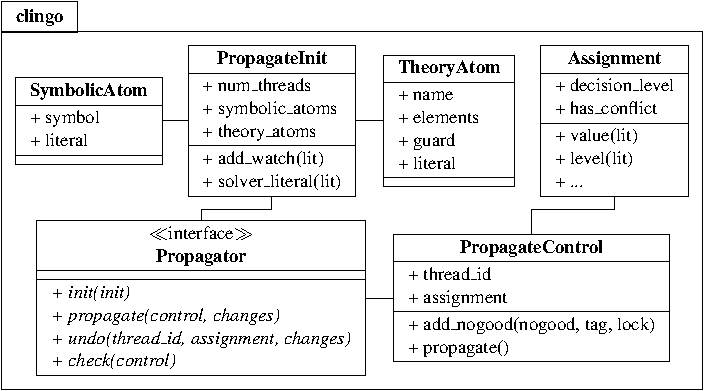
\includegraphics[width=\textwidth]{figures/python-interface}
  \caption{Class diagram of \clingo's (theory) propagator interface\label{fig:interface}}
\end{figure}
%
%
The interface \code{Propagator} has to be implemented by each custom propagator.
After registering such a propagator with \clingo,
its functions are called during initialization and search as indicated %
in Figure~\ref{fig:cdcl}.
%
Function \code{Propagator.init}%
\footnote{For brevity, we below drop the qualification \code{Propagator} and use its function names unqualified.}
is called once before solving (Line~(\ref{fig:cdcl:init}) in Figure~\ref{fig:cdcl})
to allow for initializing data structures used during theory propagation.
It is invoked with a \code{PropagateInit} object providing access to symbolic (\code{SymbolicAtom}) as well as theory (\code{TheoryAtom}) atoms.
Both kinds of atoms are associated with program literals,\footnote{Program literals are also used in the \aspif\ format (see~\cite{gekakaosscwa16b}).} %
which are in turn associated with solver literals.%
\footnote{Note that \clasp's preprocessor might associate a positive or even negative solver literal with multiple atoms.}
Program as well as solver literals are identified by non-zero integers, where positive and negative numbers represent positive or  negative literals, respectively.
In order to get notified about assignment changes, a propagator can set up watches on solver literals during initialization.

During search, function \codeClass{Propagator}{propagate} is called with a \code{PropagateControl} object
and a (non-empty) list of watched literals that got assigned in the recent round of unit propagation (Line~(\ref{fig:cdcl:propagate}) in Figure~\ref{fig:cdcl}).
The \code{PropagateControl} object can be used to inspect the current assignment, record nogoods, and trigger unit propagation.
Furthermore, to support multi-threaded solving,
its \code{thread\_id} property identifies the currently active thread,
each of which can be viewed as an independent instance of the CDCL algorithm in Figure~\ref{fig:cdcl}.%
%
\footnote{%
Depending on the configuration of \clasp, threads can communicate with each other.
For example, some of the recorded nogoods can be shared.
This is transparent from the perspective of theory propagators.}
%
Function \codeClass{Propagator}{undo} is the counterpart of \codeClass{Propagator}{propagate}
and called whenever the solver retracts assignments to watched literals (Line~(\ref{fig:cdcl:undo}) in Figure~\ref{fig:cdcl}).
In addition to the list of watched literals that have been retracted (in chronological order),
it receives the identifier and the assignment of the active thread.
%
Finally, function \codeClass{Propagator}{check} is similar to \codeClass{Propagator}{propagate},
yet invoked without a list of changes.
Instead, it is (only) called on total assignments
(Line~(\ref{fig:cdcl:check}) in Figure~\ref{fig:cdcl}), independently of watches.
%
Overriding the empty default implementations of propagator methods is optional.
%
For brevity, we below focus on implementations of the methods in \python,
while \lua\ or \C\ could be used as well.

For illustration,
consider Listing~\ref{prg:pigeon:propagator} giving a propagator for (half of) the pigeon-hole problem.
%
\lstinputlisting[linerange={1-10,12-39},float=t,mathescape=true,escapeinside={\#(}{\#)},basicstyle={\ttfamily\small},label={prg:pigeon:propagator},caption={Propagator for the pigeon-hole problem},language=clingo]{example/pigeon-py.lp}
%
Although this setting is constructed, it showcases central aspects
that are also relevant when implementing more complex propagators,
e.g., the \code{Pigeonator} is both stateful and can be used with multiple threads.
%
The underlying ASP encoding is given in Line~\ref{prg:pigeon:prop:rule1}:
A (choice) rule generates solution candidates by placing each of the $p$ pigeons in exactly one among $h$ holes.
While the rule commented out in Line~\ref{prg:pigeon:prop:rule2} would ensure that there is at most one pigeon per hole,
this constraint is handled by the \code{Pigeonator} class
implementing the \code{Propagator} interface (except for \code{check}) in Lines~\ref{prg:pigeon:prop:begin-init}--\ref{prg:pigeon:prop:end-undo}.
Whenever two pigeons are placed in the same hole, it adds a binary nogood forbidding the placement.
To this end,
it maintains data structures for, given a newly placed pigeon,
detecting whether there is a conflict.
%
More precisely, the propagator has two data members:
The \code{self.place} dictionary in Line~\ref{prg:pigeon:prop:member-place} maps solver literals
for \code{place}$/2$ atoms to their corresponding holes,
and the \code{self.state} list in Line~\ref{prg:pigeon:prop:member-state} stores for each solver thread its current placement of pigeons
as a mapping from holes to true solver literals for \code{place}$/2$ atoms.

Function \codeClass{Pigeonator}{init} in Lines~\ref{prg:pigeon:prop:begin-init}--\ref{prg:pigeon:prop:end-init}
sets up watches as well as the dictionaries in \code{self.place} and \code{self.state}.
%
To this end,
it traverses (symbolic) atoms over \code{place}$/2$ in Lines~\ref{prg:pigeon:prop:init:loop-atoms}--\ref{prg:pigeon:prop:init:end-loop-atoms}.
Each such atom is associated with a solver literal, %
obtained in Line~\ref{prg:pigeon:prop:init:map-literal}.
The mapping from the solver literal to its corresponding hole is then stored in the \code{self.place} dictionary in
Line~\ref{prg:pigeon:prop:init:map-lit-hole}.
%
In the last line of the loop, a watch is added for each solver literal at hand,
so that the solver calls \code{propagate} whenever a pigeon is placed. %
%
Finally, in Line~\ref{prg:pigeon:prop:init:state}, the \code{self.state} list
of placements per thread,
subject to change upon propagation and backjumping,
%
is initialized with empty dictionaries.

Function \codeClass{Pigeonator}{propagate}, given in Lines~\ref{prg:pigeon:prop:begin-prop}--\ref{prg:pigeon:prop:end-prop},
accesses \code{control.thread\_id} in Line~\ref{prg:pigeon:prop:prop:state}
to obtain the \code{holes} dictionary storing the active thread's current placement of pigeons.
%
%
The loop in Lines~\ref{prg:pigeon:prop:prop:begin-loop}--\ref{prg:pigeon:prop:prop:end-loop} then iterates over the list of changes,
i.e., solver literals representing newly placed pigeons.
After in Line~\ref{prg:pigeon:prop:prop:pigeon-to-hole}
determining the \code{hole} associated with a recently assigned literal,
%
%
\python's \code{setdefault} function is used to update the state:
Depending on whether \code{hole} already appears as a key in the \code{holes} dictionary,
the function either retrieves its associated literal or inserts the new literal under key \code{hole}. %
While the latter case amounts to updating the placement of pigeons, the former signals a conflict,
triggered by recording a binary nogood in Line~\ref{prg:pigeon:prop:prop:add-clause}.
%
Given that the solver has to resolve the conflict and backjump,
the call to \code{add\_nogood} always yields false, so that
propagation stops without processing remaining changes any further.\footnote{%
  The optional arguments \code{tag} and \code{lock} of \code{add\_nogood} can be used to control the scope and lifetime of recorded nogoods.
  Furthermore, in a propagator that does not add violated nogoods only, %
  function \code{control.propagate} can be invoked to trigger unit propagation.
  }


Function \codeClass{Pigeonator}{undo} in Lines~\ref{prg:pigeon:prop:begin-undo}--\ref{prg:pigeon:prop:end-undo} resets a thread's placement of pigeons upon backjumping.
Similar to \codeClass{Pigeonator}{propagate}, %
the active thread's current placement
is obtained in Line~\ref{prg:pigeon:prop:undo:state},
and changes are traversed in Lines~\ref{prg:pigeon:prop:undo:begin-loop}--\ref{prg:pigeon:prop:undo:del}.
%
%
The latter correspond to retracted solver literals,
for which the condition in Line~\ref{prg:pigeon:prop:undo:test} makes sure
that exactly those stored in Line~\ref{prg:pigeon:prop:prop:setdefault} before are cleared,
thus reflecting that the \code{hole} determined in Line~\ref{prg:pigeon:prop:undo:pigeon-to-hole}
is free again.
%
Finally,
function \code{main} in Lines~\ref{prg:pigeon:prop:begin-main}--\ref{prg:pigeon:prop:end-main} first registers the \code{Pigeonator} propagator in Line~\ref{prg:pigeon:prop:register},
and then initiates grounding and solving with \clingo.


\section{Experiments}\label{sec:experiments}
\newcommand{\TO}{\multicolumn{1}{r|}{TO}}
\newcommand{\TI}{\multicolumn{1}{r|}{T}}

Our approach aims at a simple yet general framework for incorporating theory reasoning into ASP solving.
Hence, it leaves room for various ways of encoding a problem and of implementing theory propagation.
%
To reflect this from a practical perspective,
we empirically explore several options for solving problems with difference logic (\DL) constraints.
%
To be more precise,
we contrast an encoding relying on \emph{defined} theory atoms with one leaving them \emph{external} (cf.\ Section~\ref{sec:foundations}),
and a \emph{stateless} with a \emph{stateful} propagator implementation.
As a \emph{non-strict} interpretation of \DL\ constraints is sufficient
for the problems given below,
we stick to this option and do not vary it.

The consistency of a set $C$ of \DL\ constraints can be checked by mapping them to a weighted directed graph $G(C)$.
The nodes of $G(C)$ are the (integer) variables occurring in $C$,
and for each $x_1 - x_2 \leq k$ in $C$, $G(C)$ includes an edge from $x_1$ to $x_2$ with weight $k$.
Then, $C$ is \DL-consistent iff $G(C)$ contains no cycle whose sum of edge weights is negative.
%
The difference between a stateless and stateful \DL-propagator amounts to whether the corresponding graph is
built from scratch upon each invocation or only once and updated subsequently.
%
In our experiments,
we use the Bellman-Ford algorithm \cite{bellman58a,forful62a} as basis for a stateless propagator,
and the one in \cite{cotmal06a} for update operations in the stateful case.
%
Both propagator implementations detect negative cycles
and record (solver) literals corresponding to their weighted edges as nogoods.

Theory atoms corresponding to \DL\ constraints are formed as described in Section~\ref{sec:language}.
%
The difference between using defined and external theory atoms boils down to their occurrence in the head of a rule,
as in Line~\ref{prg:diff:rule-diff} of Listing~\ref{prg:diff}, viz.\
\begin{lstlisting}[morekeywords={&diff},alsoletter={\&},numbers=none]
&diff { end(T)-start(T) } <= D :- duration(T,D).
\end{lstlisting}
or in the body, as in
\begin{lstlisting}[morekeywords={&diff},alsoletter={\&},numbers=none]
:- duration(T,D), not &diff { end(T)-start(T) } <= D.
\end{lstlisting}
%
Note that the defining usage constrains \DL-atoms firmer than the external one:
A defined \DL-atom is true iff at least one of its bodies holds,
while an external one may vary whenever its truth is \DL-consistent yet
not imposed by integrity constraints (with further problem-specific literals).

To evaluate the different options,
we expressed (decision versions of) several scheduling problems \cite{taillard93a},
typically aiming at the minimization of schedules' makespan,
by logic programs in the language of Section~\ref{sec:language}.
%
\emph{Flow shop}:
A schedule corresponds to a permutation of~$n$ jobs,
each including $m$ sequential subtasks allocating
machines $1,\dots, m$ for specific amounts of time.
%
\emph{Job shop}:
Again considering~$n$ jobs with $m$ sequential subtasks each,
where the order in which subtasks allocate machines $1,\dots, m$ for given amounts of time
is job-specific,
a schedule arranges the subtasks of different jobs in one sequence per machine.
%
\emph{Open shop}:
Given the same setting as in the job shop problem,
the sequential order of the subtasks of a job is not fixed,
but augments a schedule arranging the subtasks of different jobs per machine.
%
For reasons of scalability,
we refrain from optimizing the makespan of schedules,
but are only interested in some feasible schedule per instance along with
the corresponding earliest start times of subtasks.

\begin{table}
\caption{Comparison between different encodings and \DL-propagators for scheduling problems}
\centering
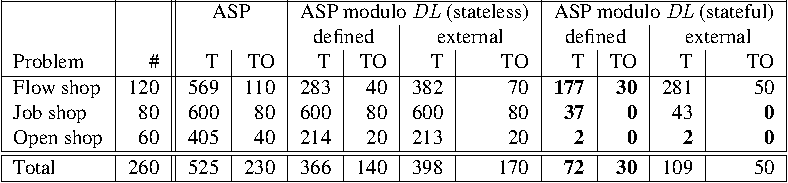
\includegraphics{tables/shop-scheduling}
\label{table:bench:encoding_comparisson}
\end{table}
The results of our experiments,
run sequentially under Linux on an Intel Xeon E5520 2.27~GHz machine equipped with 24~GB main memory,
are summarized in Table~\ref{table:bench:encoding_comparisson}.
%
%
Each \clingo~5 run was restricted to 600 seconds wall-clock time, while memory was never exceeded.
%
Subcolumns headed by  `T'  report average runtimes, taking timeouts as 600~seconds, and
those with  `TO'  numbers of timeouts over  `\#'  instances of each scheduling problem and
in total.
Respective results in the column headed by  `ASP'
reflect the bottom-line performance obtained with plain ASP encodings,
which is obviously not competitive due to the ineffectiveness of grounding
problems over large numeric domains.
%
The remaining columns consider the four combinations of encoding and \DL-propagator features of interest.
%
First,
we observe that the stateful propagator (on the right) has a clear edge over its stateless counterpart
(in the middle).
Second,
with both propagator implementations,
the firm encoding using defined \DL-atoms outperforms the one leaving them external
on instances of the flow shop problem.
%
While this experiment is not meant to be universal,
it demonstrates that different features have an impact on the resulting performance.
%
In how far the tuning of theory propagators matters also depends on the use case at hand, e.g.,
solving a challenging application problem  versus rapid prototyping of dedicated reasoning procedures.

\section{Discussion}\label{sec:discussion}

The \clingo~5 system provides a comprehensive infrastructure for enhancing ASP with theory reasoning.
This ranges from
generic means for expressing theories along with their support by \gringo,
over a theory-aware intermediate format,
to simple yet powerful interfaces in \C, \lua, and \python.
In each case, a propagator can    specify (up to) four basic functions to customize its integration into \clasp's propagation,
where an arbitrary number of (independent) theory propagators can be be incorporated.
%
Logically, ASP encodings may build upon defined or external theory atoms,
and their associated conditions may be strict or non-strict.
In practice,
\clingo~5 supports stateless and stateful theory propagators, which can be controlled in a fine-grained way.
%
For instance, propagators are thread-sensitive, watches can be set to symbolic as well as theory literals,
and the scope and lifetime of nogoods stemming from theory propagation can be configured.

A first step toward a more flexible ASP infrastructure
was done with \clingo~4 \cite{gekakasc14b} by introducing \lua\ and \python\ APIs for multi-shot solving.
Although this allows for fine-grained control of complex ASP reasoning processes,
the functionality provided no access to \clasp's propagation and was restricted to inspecting (total) stable models.
%
The extended framework for theory propagation relative to partial assignments (cf.\ Figure~\ref{fig:cdcl})
follows the canonical approach of SMT \cite{baseseti09a}.
%
%
While \dlvhex\ implicitly provides access to \clasp's propagation,
this is done on the more abstract level of higher-order logic programs.
Also, \dlvhex\ as well as many other systems, such as \clingcon\ or \inca,
implement specialized propagation via \clasp's internal interfaces,
whose usage is more involved and subject to change with each release.
%
Although the new high-level interfaces may not yet fully cover all desired features,
they provide a first step toward easing the development of such dedicated systems and
putting them on a more stable basis.
%
Currently,
\clingo~5's infrastructure is already used as a basis for
\clingcon~3 \cite{bakakaossc16a},
%
\lctocasp\ \cite{cakaossc16a},
and
its integration with SWI-Prolog.
%
Finally, we believe that the extended grounding capacities along with the intermediate format supplemented in~\cite{gekakaosscwa16b}  %
will also be beneficial for non-native approaches and ease the overall development of ASP-oriented solvers.
This applies to systems like \dingo, \mingo, and \aspmt\ \cite{barlee14b},
the latter implementing ASP with theory reasoning by translation to SMT,
which so far had to resort to specific input formats and meta-programming to bypass the grounder.

\bibliography{Gebser}

\end{document}

%%% Local Variables:
%%% mode: latex
%%% TeX-master: t
%%% End:
